\setcounter{ExampleCounter}{1}
We can use sets to organize the results of a survey by visualizing the respondents with a Venn diagram.  Specifically, if a survey asks more than one question, a Venn diagram can be a really handy tool.

\begin{example}{Movie Types}
Brianne surveyed students in her school to determine what types of movies they prefer: science fiction, comedy, both types of movies, or neither type of movie.  If $A$ represents science fiction and $B$ represents comedy, the following diagram shows the result of her survey.

\begin{center}
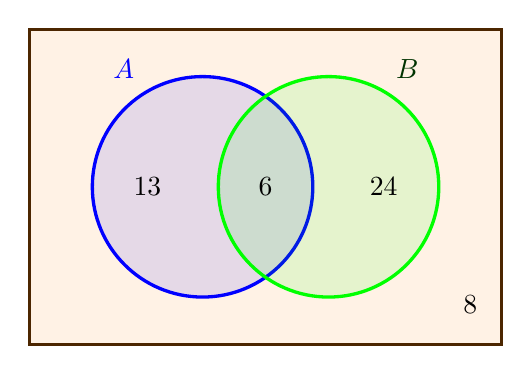
\begin{tikzpicture}
  \draw [very thick,color=orange!30!black, fill=orange!10] (-3cm,-2cm) rectangle (3cm,2cm);

  \draw [very thick,color=blue, fill=blue, fill opacity=0.1] (-0.8,0) circle (1.4cm);
  \draw [very thick,color=green, fill=green, fill opacity=0.1] (0.8,0) circle (1.4cm);
  \draw [yshift=1.5cm,xshift=-1.8cm] node {\color{blue} $A$};
  \draw [yshift=1.5cm,xshift=1.8cm] node {\color{green!20!black} $B$};
  
  \draw [yshift=0cm,xshift=0cm] node {6};
  \draw [yshift=0cm,xshift=-1.5cm] node {13};
  \draw [yshift=0cm,xshift=1.5cm] node {24};
  \draw [yshift=-1.5cm,xshift=2.6cm] node {8};
  
  
  
  %\draw [ultra thick, color=red] (-1.4,0) ++(45:2) arc (45:315:2);
  %\draw [ultra thick, color=red] (1.4,0) ++(135:2) arc (135:-135:2);
  
  %\draw [ultra thick,color=blue!20!green!10!white] (0,-1.414) -- (0,1.414);
  %\draw [ultra thick,color=blue,fill=blue!20!green!10!white] (-1.4,0) ++(45:2) arc (45:-45:2);
  %\draw [ultra thick,color=green,fill=blue!20!green!10!white] (1.4,0) ++(135:2) arc (135:225:2);
  %\draw [ultra thick, color=red] (-1.4,0) ++(45:2) arc (45:315:2);
  %\draw [ultra thick, color=red] (1.4,0) ++(135:2) arc (135:-135:2);
  %\draw [yshift=0cm,xshift=0cm] node {\color{red!20!black} $A \cap B$};
  
  %\draw [yshift=-3.5cm,xshift=0cm] node {$(A \cup B)^c = A^c \cap B^c$};
  
\end{tikzpicture}
\end{center}

Answer the following questions.
\begin{enumerate}[(a)]
\item How many students did Brianne survey?
\item How many students like science fiction?
\item How many students like \textbf{only} science fiction?
\item How many students like comedy?
\item How many students like comedy, but not science fiction?
\item How many like both science fiction and comedy?
\item How many like science fiction or comedy?
\item How many like neither?
\item How many do not like science fiction?
\item How many do not like comedy?
\end{enumerate}

\sol
\begin{enumerate}[(a)]
\item How many students did Brianne survey?

This includes everyone in the universal set; the number of people in this set is the sum of all the numbers that are shown:
\[13+6+24+8 = \boxed{51}\]
Therefore, she surveyed a total of 51 students.\\

\item How many students like science fiction?

The total number of students who like science fiction is all those that are in the blue circle:
\[13+6 = \boxed{19}\]
There are 19 students who like science fiction.\\

\item How many students like \textbf{only} science fiction?

This is all those in the blue circle that are NOT also in the green circle, for a total of $\boxed{13}$\\

\item How many students like comedy?

Similarly, there are \[24+6 = \boxed{30}\] students who like comedy.\\

\item How many students like comedy, but not science fiction?

This is all those in the green circle but outside the blue circle; there are $\boxed{24}$ of these students.\\

\item How many like both science fiction and comedy?

Those who like both lie in the intersection of the two sets; there are $\boxed{6}$ of these.\\

\item How many like science fiction or comedy?

The word OR indicates that this represents the union of these two sets: there are \[13+6+24 = \boxed{43}\] students who like science fiction or comedy.\\

\item How many like neither?

This would be the $\boxed{8}$ students outside of both circles.\\

\item How many do not like science fiction?

There are two ways to do this.  On the one hand, we could add up all the numbers outside the blue circle.  On the other, we could subtract those who like science fiction (from part b) from the total number who were surveyed (from part a).  Either way, we find that there are $\boxed{32}$ students who do not like science fiction.\\

\item How many do not like comedy?

We can solve this one in a similar way; there are $\boxed{21}$ students who do not like comedy.
\end{enumerate}
\end{example}

\begin{try}
A survey asked 100 people two questions: ``Do you like M\&Ms?'' and ``Do you like Skittles?''  The results are shown below.

\begin{center}
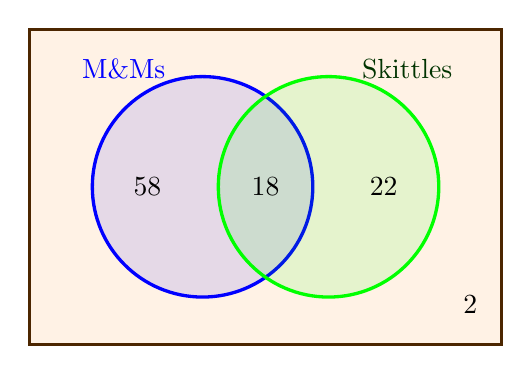
\begin{tikzpicture}
  \draw [very thick,color=orange!30!black, fill=orange!10] (-3cm,-2cm) rectangle (3cm,2cm);

  \draw [very thick,color=blue, fill=blue, fill opacity=0.1] (-0.8,0) circle (1.4cm);
  \draw [very thick,color=green, fill=green, fill opacity=0.1] (0.8,0) circle (1.4cm);
  \draw [yshift=1.5cm,xshift=-1.8cm] node {\color{blue} M\&Ms};
  \draw [yshift=1.5cm,xshift=1.8cm] node {\color{green!20!black} Skittles};
  
  \draw [yshift=0cm,xshift=0cm] node {18};
  \draw [yshift=0cm,xshift=-1.5cm] node {58};
  \draw [yshift=0cm,xshift=1.5cm] node {22};
  \draw [yshift=-1.5cm,xshift=2.6cm] node {2};
  
\end{tikzpicture}
\end{center}

\begin{enumerate}[(a)]
\item How many people liked M\&Ms, but not Skittles?
\item How many people liked Skittles?
\item How many people like M\&Ms or Skittles?
\end{enumerate}
\end{try}

If the results of a survey are not given as a Venn diagram, we can still build one to visualize the results.

\begin{example}{Travel Destinations}
Of the students in Latoya's class, eight have been to California, nine have been to Washington, and five have been to both California and Washington.  How many students have been to California or Washington?

\sol
We can draw a diagram like in the previous example to answer this question:

\begin{center}
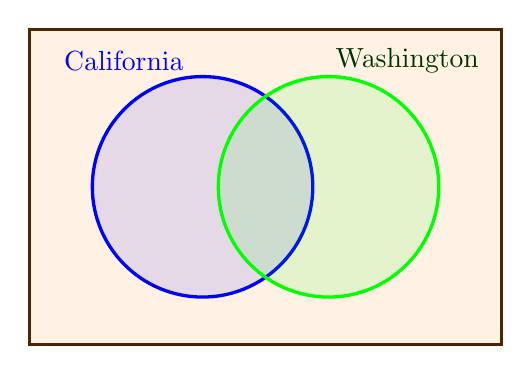
\begin{tikzpicture}
  \draw [very thick,color=orange!30!black, fill=orange!10] (-3cm,-2cm) rectangle (3cm,2cm);

  \draw [very thick,color=blue, fill=blue, fill opacity=0.1] (-0.8,0) circle (1.4cm);
  \draw [very thick,color=green, fill=green, fill opacity=0.1] (0.8,0) circle (1.4cm);
  \draw [yshift=1.6cm,xshift=-1.8cm] node {\color{blue} California};
  \draw [yshift=1.6cm,xshift=1.8cm] node {\color{green!20!black} Washington};
  
\end{tikzpicture}
\end{center}

Here's how to fill this in: \textbf{start with the innermost intersection}.  The overlap represents those who have been to both states, of which there are five.\\

Then, we know that a total of eight students have been to California; we've already accounted for five of them in the overlap, so there are three students in the left circle but NOT in the right circle.  Similarly, there are a total of nine students who have been to California, of which five have already been accounted for, leaving four others in the right circle.

\begin{center}
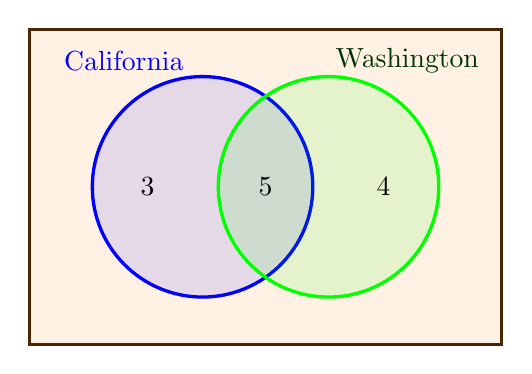
\begin{tikzpicture}
  \draw [very thick,color=orange!30!black, fill=orange!10] (-3cm,-2cm) rectangle (3cm,2cm);

  \draw [very thick,color=blue, fill=blue, fill opacity=0.1] (-0.8,0) circle (1.4cm);
  \draw [very thick,color=green, fill=green, fill opacity=0.1] (0.8,0) circle (1.4cm);
  \draw [yshift=1.6cm,xshift=-1.8cm] node {\color{blue} California};
  \draw [yshift=1.6cm,xshift=1.8cm] node {\color{green!20!black} Washington};
  
  \draw [yshift=0cm,xshift=0cm] node {5};
  \draw [yshift=0cm,xshift=-1.5cm] node {3};
  \draw [yshift=0cm,xshift=1.5cm] node {4};
  %\draw [yshift=-1.5cm,xshift=2.6cm] node {2};
  
\end{tikzpicture}
\end{center}

Finally, we can answer the question: there are a total of $\boxed{12}$ students (in the union of the two sets) who have been to either California or Washington.

\end{example}

\begin{try}
Of the children in Sofia's class, seven like to use markers, five like to use colored pencils, and three like to use both.  How many children like to use colored pencils but not markers?
\end{try}

In examples like that one with only two categories, we could potentially answer the question without drawing a diagram, but drawing the diagram becomes more and more helpful for more complicated questions, like those with three categories.
\vfill
\pagebreak

\begin{example}{TV Networks}
A survey of 125 people was conducted to determine the popularity of HBO, CNN, and MTV.  The survey found that 71 people watch HBO, 72 watch CNN, and 80 watch MTV.  Furthermore, 33 watch HBO and CNN, 42 watch HBO and MTV, and 47 watch CNN and MTV.  Finally, 11 watch all three.\\

Fill in the Venn diagram below.

\begin{center}
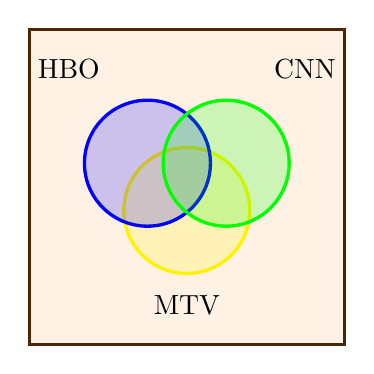
\begin{tikzpicture}
  \draw [very thick,color=orange!30!black, fill=orange, fill opacity=0.1] (-2cm,-2cm) rectangle (2cm,2cm);

  \draw [very thick,color=yellow, fill=yellow, fill opacity=0.2] (0,-0.3) circle (0.8cm);
  \draw [very thick,color=blue, fill=blue, fill opacity=0.2] (-0.5,0.3) circle (0.8cm);
  \draw [very thick,color=green, fill=green, fill opacity=0.2] (0.5,0.3) circle (0.8cm);
  
  \draw [yshift=1.5cm,xshift=-1.5cm] node {HBO};
  \draw [yshift=1.5cm,xshift=1.5cm] node {CNN};
  \draw [yshift=-1.5cm,xshift=0cm] node {MTV};
  
  %\draw [yshift=-5.75cm,xshift=0cm] node {$A \cap (B \cup C) = (A \cap B) \cup (A \cap C)$};
  
  %\node (a) at (0.5,-0.5) {};
  %\node (b) at (-0.5,-0.5) {};
  %\node (c) at (0,-1.37) {};
  %\draw [ultra thick,fill=red!20,red!20] (a.center) -- (b.center) -- (c.center) -- (a.center) -- cycle;
  
  %\draw [ultra thick,color=red,fill=red!20] (-1.4,0) ++(314:2) node(c){} arc (314:346:2);
  %\draw [ultra thick,color=red,fill=red!20] (1.4,0) ++(194:2) node(b){} arc (194:226:2);
  %\draw [ultra thick,color=red,fill=red!20] (0,-2.425) ++(74:2) node(a){} arc (74:106:2);
  
  %\draw [ultra thick,color=red!20] (0,-1.414) -- (0,1.414);
  %\draw [ultra thick,color=red,fill=red!20] (-1.4,0) ++(45:2) arc (45:-45:2);
  %\draw [ultra thick,color=red,fill=red!20] (1.4,0) ++(134:2) arc (134:226:2);
  
  
  %\draw [ultra thick,color=red,fill=red!20] (0,-2.425) ++(75:2) node(b){} arc (75:165:2) node(a){};
  %\draw [ultra thick,color=red,fill=red!20] (-1.4,0) ++(-15:2) arc (-15:-105:2);
  %\draw [ultra thick,color=red!20] (b) -- (a.center);
  %\draw [ultra thick,color=red,fill=red!20] (0,-2.425) ++(74:2) arc (74:166:2);
  
  %\draw [thick,color=red!20] (0,-1.2) -- (0,0);
  %\draw [color=red!20,fill=red!20] (-1.4,0) ++(45:1.965) arc (45:-45:1.965);
  %\draw [color=red!20,fill=red!20] (1.4,0) ++(135:1.965) arc (135:225:1.965);
  
\end{tikzpicture}
\end{center}

\sol
As before, start with the innermost intersection and work outwards.  There are 11 in the center, and a total of 33 in the intersection of HBO and CNN, so there are 22 in the intersection of HBO and CNN, but outside the center.  Go on and fill in the other two intersections, and then subtract to fill in the rest of the circles.

\begin{center}
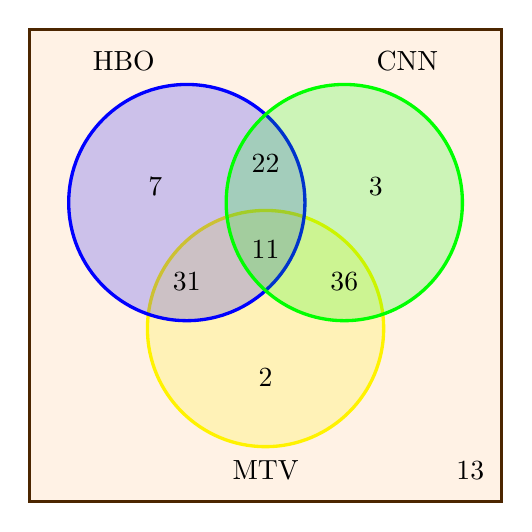
\begin{tikzpicture}
  \draw [very thick,color=orange!30!black, fill=orange, fill opacity=0.1] (-3cm,-3cm) rectangle (3cm,3cm);

  \draw [very thick,color=yellow, fill=yellow, fill opacity=0.2] (0,-0.8) circle (1.5cm);
  \draw [very thick,color=blue, fill=blue, fill opacity=0.2] (-1,0.8) circle (1.5cm);
  \draw [very thick,color=green, fill=green, fill opacity=0.2] (1,0.8) circle (1.5cm);
  
  \draw [yshift=2.6cm,xshift=-1.8cm] node {HBO};
  \draw [yshift=2.6cm,xshift=1.8cm] node {CNN};
  \draw [yshift=-2.6cm,xshift=0cm] node {MTV};
  
  %\draw [very thick,color=orange!30!black, fill=orange, fill opacity=0.1] (-4cm,-5.4cm) rectangle (4cm,3cm);

  %\draw [very thick,color=yellow, fill=yellow, fill opacity=0.2] (0,-2.425) circle (2cm);
  %\draw [very thick,color=blue, fill=blue, fill opacity=0.2] (-1.4,0) circle (2cm);
  %\draw [very thick,color=green, fill=green, fill opacity=0.2] (1.4,0) circle (2cm);
  
  %\draw [yshift=2.6cm,xshift=-1.8cm] node {HBO};
  %\draw [yshift=2.6cm,xshift=1.8cm] node {CNN};
  %\draw [yshift=-5cm,xshift=0cm] node {MTV};
  
  \draw [yshift=0.2cm,xshift=0cm] node {11};
  \draw [yshift=1.3cm,xshift=0cm] node {22};
  \draw [yshift=-0.2cm,xshift=1cm] node {36};
  \draw [yshift=-0.2cm,xshift=-1cm] node {31};
  \draw [yshift=1cm,xshift=-1.4cm] node {7};
  \draw [yshift=1cm,xshift=1.4cm] node {3};
  \draw [yshift=-1.425cm,xshift=0cm] node {2};
  \draw [yshift=-2.6cm,xshift=2.6cm] node {13};
  
  %\draw [yshift=-5.75cm,xshift=0cm] node {$A \cap (B \cup C) = (A \cap B) \cup (A \cap C)$};
  
  %\node (a) at (0.5,-0.5) {};
  %\node (b) at (-0.5,-0.5) {};
  %\node (c) at (0,-1.37) {};
  %\draw [ultra thick,fill=red!20,red!20] (a.center) -- (b.center) -- (c.center) -- (a.center) -- cycle;
  
  %\draw [ultra thick,color=red,fill=red!20] (-1.4,0) ++(314:2) node(c){} arc (314:346:2);
  %\draw [ultra thick,color=red,fill=red!20] (1.4,0) ++(194:2) node(b){} arc (194:226:2);
  %\draw [ultra thick,color=red,fill=red!20] (0,-2.425) ++(74:2) node(a){} arc (74:106:2);
  
  %\draw [ultra thick,color=red!20] (0,-1.414) -- (0,1.414);
  %\draw [ultra thick,color=red,fill=red!20] (-1.4,0) ++(45:2) arc (45:-45:2);
  %\draw [ultra thick,color=red,fill=red!20] (1.4,0) ++(134:2) arc (134:226:2);
  
  
  %\draw [ultra thick,color=red,fill=red!20] (0,-2.425) ++(75:2) node(b){} arc (75:165:2) node(a){};
  %\draw [ultra thick,color=red,fill=red!20] (-1.4,0) ++(-15:2) arc (-15:-105:2);
  %\draw [ultra thick,color=red!20] (b) -- (a.center);
  %\draw [ultra thick,color=red,fill=red!20] (0,-2.425) ++(74:2) arc (74:166:2);
  
  %\draw [thick,color=red!20] (0,-1.2) -- (0,0);
  %\draw [color=red!20,fill=red!20] (-1.4,0) ++(45:1.965) arc (45:-45:1.965);
  %\draw [color=red!20,fill=red!20] (1.4,0) ++(135:1.965) arc (135:225:1.965);
  
\end{tikzpicture}
\end{center}

Now that we have the Venn diagram, we can answer questions like the following ones.

\begin{enumerate}[(a)]
\item How many watch only MTV?
\[\boxed{2}\]
\item How many watch CNN and MTV, but not HBO?
\[\boxed{36}\]
\item How many do not watch any of these networks?
\[\boxed{13}\]
\item How many do not watch CNN?
\[\boxed{53}\]
\item How many watch HBO or MTV?
\[\boxed{109}\]
\end{enumerate}

\end{example}

\begin{try}
Fifty students were surveyed and asked if they were taking a social science, humanities, or natural science course the next semester.\\

The survey found that 21 were taking a social science course, 26 were taking humanities, 19 were taking natural science.  Also, 9 were taking social science and humanities, 7 were taking social science and natural science, and 10 were taking humanities and natural science.  Finally, 3 students were taking all three.

\begin{enumerate}[(a)]
\item How many students are taking only a social science course?
\item How many are taking natural science and social science, but not humanities?
\item How many are taking none of these courses?
\end{enumerate}
\end{try}

\begin{example}{Comcast Services}
A survey of 1000 households found that 470 use Comcast internet service, 420 use their telephone service, and 319 use their cable television.  Of these, 140 families use the telephone and television services, 220 families use the internet and television service, and 110 use the internet and telephone.  There are 75 families who use all three.

The diagram below summarizes this information.

\begin{center}
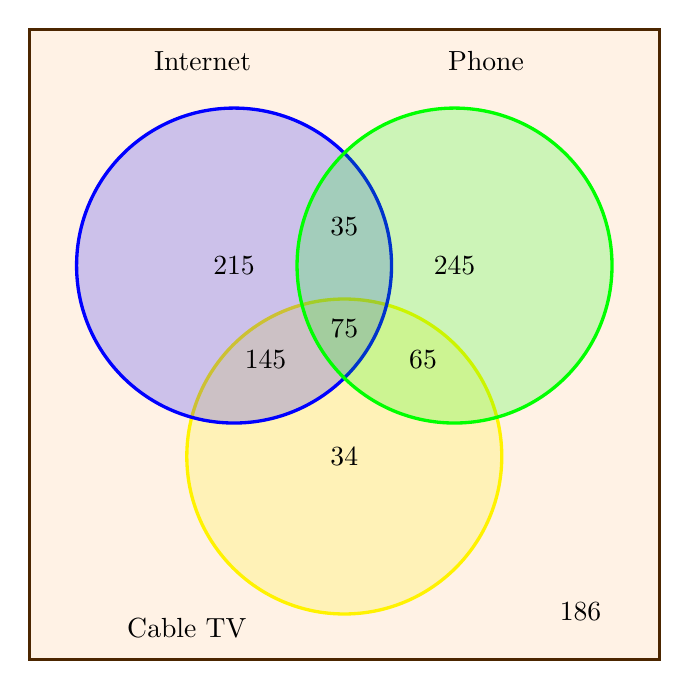
\begin{tikzpicture}
  \draw [very thick,color=orange!30!black, fill=orange, fill opacity=0.1] (-4cm,-5cm) rectangle (4cm,3cm);

  \draw [very thick,color=yellow, fill=yellow, fill opacity=0.2] (0,-2.425) circle (2cm);
  \draw [very thick,color=blue, fill=blue, fill opacity=0.2] (-1.4,0) circle (2cm);
  \draw [very thick,color=green, fill=green, fill opacity=0.2] (1.4,0) circle (2cm);
  
  \draw [yshift=2.6cm,xshift=-1.8cm] node {Internet};
  \draw [yshift=2.6cm,xshift=1.8cm] node {Phone};
  \draw [yshift=-4.6cm,xshift=-2cm] node {Cable TV};
  
  \draw [yshift=-0.8cm,xshift=0cm] node {75};
  \draw [yshift=0.5cm,xshift=0cm] node {35};
  \draw [yshift=-1.2cm,xshift=1cm] node {65};
  \draw [yshift=-1.2cm,xshift=-1cm] node {145};
  \draw [yshift=0cm,xshift=-1.4cm] node {215};
  \draw [yshift=0cm,xshift=1.4cm] node {245};
  \draw [yshift=-2.425cm,xshift=0cm] node {34};
  \draw [yshift=-4.4cm,xshift=3cm] node {186};
  
\end{tikzpicture}
\end{center}

\begin{enumerate}
\item How many households in this survey do not use any of these services?
\[\boxed{186}\]
\item How many use exactly one of these services?\\

These are all the ones that lie in only one circle:
\[\boxed{494}\]

\item How many use exactly two of these services?\\

These are all the ones that lie in the intersection of two circles, but not in the very center:
\[\boxed{245}\]
\end{enumerate}
\end{example}